\subsection{UC-21}
\label{subsec:UC-21}

\begin{figure}[H]
    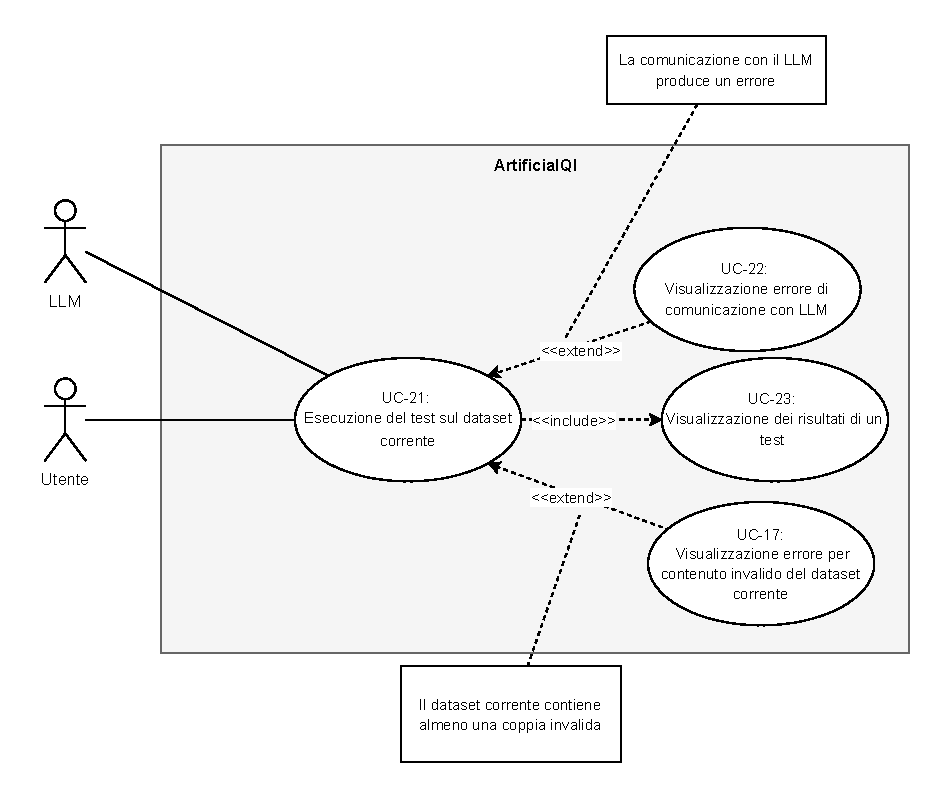
\includegraphics[scale=0.8]{Sezioni/UseCase/Immagini/UC-21.pdf}
    \caption{Diagramma UC-21.}
\end{figure}

\begin{usecase}{UC-21}{Esecuzione del test sul dataset corrente}

    \req{\hyperref[item:RU-7]{RU-7}} 

    \pre{
        \item Il sistema è attivo e funzionante
        \item Il dataset da utilizzare per l'esecuzione del test è stato caricato come dataset corrente
        \item Il dataset corrente non è vuoto
    }

    \post{
        \item L'utente conosce l'esito del test
    }
    
    \actor{Utente}

    \subactors{LLM}

    \trigger{L'utente deve testare il LLM usando il dataset corrente}
    
    \inc{\hyperref[subsec:UC-23]{UC-23}}

    \base{}

    \scenario{
        \item L'utente richiede l'esecuzione del test
        \item Per ogni coppia del dataset corrente si ottiene la risposta prodotta dal LLM sotto test
        \item Per ogni coppia del dataset corrente si calcola il grado di somiglianza tra la risposta prodotta dal LLM sotto test rispetto alla risposta attesa alla domanda della coppia
        \item \texttt{<<include:UC-23>>}
    }

    \subscenario{
        \item[1.1] \textbf{Il dataset corrente contiene almeno una coppia invalida}
        \begin{itemize}
            \item[a.] \hyperref[subsec:UC-17]{UC-17}
        \end{itemize}
        \item[2.1] \textbf{La comunicazione con LLM produce un errore}
        \begin{itemize}
        \item[a.] \hyperref[subsec:UC-22]{UC-22}
        \end{itemize}
    }
\end{usecase}